
\documentclass[11pt]{article}

\usepackage{amsmath} %import amsmath for align command
\usepackage{cite} %import package for using bibtex bibliography
\usepackage{graphicx} %import package for inserting figures from image files
\usepackage{mathtools} %import package for using certain symbols such as eq. arrows
\usepackage{tikz} %import package for creating figures
\usepackage{booktabs}
\usepackage{siunitx}
\usepackage[T1]{fontenc}
\usepackage[font=small,skip=0pt]{caption}


\usepackage{placeins}
\usepackage{array}
\newcolumntype{P}[1]{>{\centering\arraybackslash}p{#1}}

\usepackage[nodisplayskipstretch]{setspace}


\usepackage{titlesec}
\titlespacing{\section}{0pt}{0.8\baselineskip}{0.8\baselineskip}
\titlespacing{\subsection}{0pt}{0.675\baselineskip}{0.675\baselineskip}
\setlength{\abovecaptionskip}{2pt plus 2pt minus 5pt}

% for referencing links
\usepackage{hyperref}
\hypersetup{
	colorlinks=true,
	linkcolor=blue,
	filecolor=magenta,
	urlcolor=cyan,
}

% \usepackage{apacite}

\usepackage{algorithm}
\usepackage[noend]{algpseudocode}
\usepackage{textcomp}
\usepackage{subcaption}

%change default margins
\setlength{\topmargin}{-.75in}
\setlength{\textheight}{9.5in}

\setlength{\oddsidemargin}{0in}
\setlength{\evensidemargin}{0in}
\setlength{\textwidth}{6.6in}

\graphicspath{{aima/images/}}

\newcommand{\urlNewWindow}[1]{\href[pdfnewwindow=true]{#1}{\nolinkurl{#1}}}
\newcommand{\problemone}{grid world problem}
\newcommand{\Problemone}{grid world problem}
\newcommand{\problemtwo}{choice suggestion problem}
\newcommand{\Problemtwo}{choice suggestion problem}
\newcommand{\expnumber}[2]{{#1}\mathrm{e}{#2}}

\begin{document}

%create title
\title{Deep Reinforcement Learning Nanodegree\\
	   Project 2 -- Continuous Control Report}
\author{\vspace{-1mm}Chris Cadonic\\
chriscadonic@gmail.com}
\maketitle
\vspace{-1.5em}

\section{Introduction}

As part of this the deep reinforcement learning nanodegree program, this report discusses my work in training an agent to continuously control an arms that aims to reach towards a certain location that changes in 3D space over time.

\subsection{Environment Overview}

The environment, called \textit{Reacher}, is a continuous control learning condition wherein an arm is tasked to reach up to have the proximal section of the arm to remain in a specified location that may move around in 3D-space. The task of the agent is to reach up and finely adjust its positioning to continue to meet the requirements of being in this location.

For this task, the environment can be summarized as follows:

\begin{table}[!ht]
	\centering
	\begin{tabular}{ c | p{10cm} }
		\textbf{MDP property} & \textbf{characteristics} \\
		\hline
		observation space & vector of length 33, containing continuous values for position, rotation, velocity, and angular velocities \\
		\hline
		action space & vector of length 4, containing continuous values for torque to be applied to two arm joints \\
		\hline
		rewards & +0.01 for each step the agent's hand is in the target location \\
		\hline
	\end{tabular}
	\caption{Hyperparameters experimented with to train an agent using DQN.}
	\label{tbl:mdp}
\end{table}

\FloatBarrier

With these characteristics, the agent can learn how to maximize the amount of reward by adjusting joint torques such that it learns how to keep it's hand in the target position as often as possible. An example image to illustrate the environment utilized for this project is shown in Figure \ref{fig:example-game-image}, where 20 separate agents are trained in parallel to learn how to properly move an arm (white) such that its hand (blue blobs) remain in the green target locations.

\begin{figure}[!ht]
	\centering
	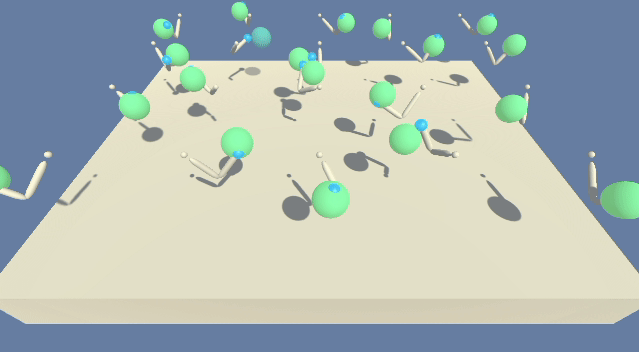
\includegraphics[width=0.75\linewidth]{images/example-env-image.png}
	\caption{A snapshot of the continuous control Unity-ML Reacher environment. White arms are agent-controlled (20 independent agents shown here), aiming to contain the blue hand in the green target locations.}
	\label{fig:example-game-image}
\end{figure}

\FloatBarrier

\section{Approach}

The overall approach used herein was to utilize the \textit{Deep Deterministic Policy Gradient} (DDPG) algorithm. This algorithm is explained in more detail in the following section.

\subsection{DDPG}

This algorithm is a policy gradient algorithm that adapts Q-learning for a continuous action space, wherein both a Q-function approximation is learned alongside a serially adapted policy. Similar to the DQN algorithm, target networks are utilized in learning both an \textit{actor} network and a \textit{critic} network drawing from experiences in an expanding experience replay buffer.

Here, the \textit{actor} network is responsible for leveraging the approximation of the Q-function to determine an optimal action per time step. In this specific instance, the Q-function is represented not as a tabular matrix, due to the continuous nature and under the assumption that the Q-function is differentiable, instead the actions are selected as a continuous maxima on the Q and utilize gradient ascent.

Additionally, the \textit{critic} network is only concerned with improving the Q-function approximation, whereby the network evaluates the value of taken actions against the value of predicted actions suggested by the \textit{actor} network.

Finally, a unique addition to the DDPG algorithm in comparison to other deep network algorithms for handling exploration vs. exploitation regards how noise is introduced to action values. The standard DDPG algorithm utilized \textit{Ornstein-Uhlenbeck} noise processes \cite{ddpg}, which is a mean-regressing noise process that results in a dampening normal noise over a time period. Specifically, over each training episode the noise injected to action values are slowly dampened over an episode to revert to noise generated around a tight Gaussian with mean 0.

\subsection{Implementation}

The specific implementation of DDPG completed in this work took two major forms, one to implement the standard DDPG algorithm as detaile din \cite{ddpg}, and another that adapts this to learn from multiple agents in parallel using a shared experience replay buffer.

The former involves the following characteristics:
\begin{itemize}
	\item both \textit{actor} and \textit{critic} networks utilized a baseline and target network pairing during training, where target networks are updated using a per-step soft-update schedule with ratio $\tau$,
	\item the \textit{actor} network seemed to benefit from a simpler architecture in comparison to the \textit{critic} network,
	\item using a repeatable update schedule per step (i.e., the networks can be updated \textit{m} times per step) along with learning rate $\alpha$,
\end{itemize}

 \FloatBarrier
 
 Using these implementation details on top of the DDPG algorithm, I settled on the following hyperparameters:
 
 \FloatBarrier
 
 \begin{table}[!ht]
 	\centering
 	\begin{tabular}{ c | p{6cm} | c }
 		\textbf{hyperparameter} & \textbf{utility} & \textbf{value} \\
 		\hline
 		$\alpha$ & learning rate & $0.001$ \\
 		$\tau$ & target network soft-update ratio & $0.001$ \\
 		$\gamma$ & discount factor on future returns & $0.99$ \\
 		$t\ update$ & number of steps to take before updating networks & $1$ \\
 		$num\ updates$ & number of updates to complete each time networks are updated during training & $2$ \\
 		$\mu$ & regression mean for Ornstein-Uhlenbeck noise & $0.0$ \\
 		$\theta$ & factor for weighing the delta of value from mean & $0.15$ \\
 		$\sigma$ & factor for weighing the Weiner (Gaussian) noise process & $0.2$ \\
 		\hline
 	\end{tabular}
 	\caption{Hyperparameters experimented with to train an agent using DQN.}
 	\label{tbl:parameters}
 \end{table}
 
 Values were either determined experimentally, such as by varying learning rate $\alpha$, $\tau$, $\gamma$, and the integers for the update schedule, or utilized from the original DDPG paper \cite{ddpg} as in the parameters for the noise process $\mu$, $\theta$, and $\sigma$.
 
  \FloatBarrier
  
  \begin{figure}[!ht]
 	\centering
 	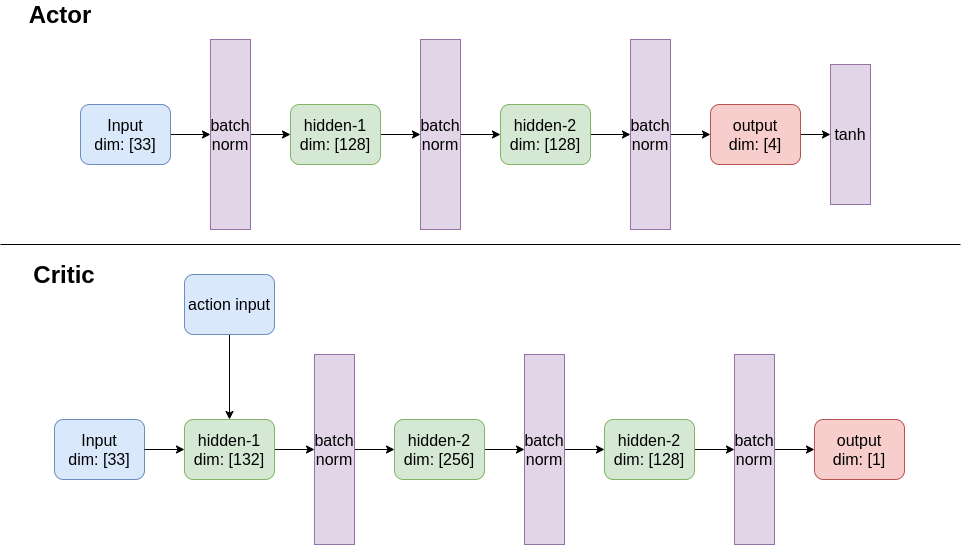
\includegraphics[width=0.8\linewidth]{images/architectures.png}
 	\caption{The architectures used in the final \textit{actor} and \textit{critic} networks in the DDPG algorithm. Though not specified, all activation functions are ReLU unless otherwise noted.}
 	\label{fig:nn-architecture}
 \end{figure}
 
 \FloatBarrier
 
 Lastly, different variations on architecture were tested, with major architectural changes primarily affecting the bound of steady-state long-term performance of the agents. For best results, it appeared that a two hidden layer \textit{actor} network and a two to three layer \textit{critic} network produced fairly stable results. Architectures are outlined above in Figure \ref{fig:nn-architecture}.
 

\section{Results and Discussion}

\subsection{Learning Performance}

After determining 

\FloatBarrier

\begin{figure}[!ht]
	\centering
	%\includegraphics[width=0.9\linewidth]{images/d4pg-results.png}
	\caption{}
	\label{fig:d4pg-results}
\end{figure}

\FloatBarrier

\subsection{Next Steps}

\section{Conclusion}

\bibliographystyle{unsrt}
\bibliography{refs}
% \begin{thebibliography}{9}
% \bibitem{littman}
% Leslie~Pack Kaelbling, Michael~L Littman, and Andrew~W Moore.
% \newblock Reinforcement learning: A survey.
% \newblock {\em Journal of artificial intelligence research}, 4:237--285, 1996.
% \end{thebibliography}

\end{document}
